\subsection{Алгоритъм за автоматично изчертаване на обобщени мрежи}
\label{sec:auto-drawing}

\hspace*{2.5em}Настоящата глава е посветена на решението на \ref{task:auto-draw}, което включва разработването на алгоритъм за автоматично изчертаване на ОМ, подробно разгледан в \cite{DimitrievTerziev}.

\subsubsection{Въведение}
\hspace*{2.5em}В практиката при работа с ОМ се наблюдава съществено предизвикателство, свързано с необходимостта от значителен ръчен труд при тяхното чертане. Традиционно в научни статии и книги ОМ се чертаят с прецизно задаване на координати за всеки елемент. Макар този подход да осигурява висока точност, той е времеемък и крие риск от човешка грешка. В \cite{IkonomovGNDraw} се разглежда изчертаване на мрежата при предварително зададена подредба на преходите и позициите, което улеснява процеса, но отново изисква ръчни настройки.

Същото затруднение се наблюдава и при ОМ симулаторите, където координатите трябва да се въвеждат ръчно, за да се визуализира мрежата. Този процес не само забавя моделирането, но и възпрепятства бързото експериментиране и прототипиране.

В отговор на това предизвикателство се предлага нов алгоритъм за автоматизирано чертане на ОМ. Той значително ускорява процеса, като генерира ясни и разбираеми визуални представяния на мрежите само на базата на тяхното абстрактно описание. Чрез елиминиране на необходимостта от ръчно задаване на координати, предложеният подход улеснява създаването и манипулирането на ОМ и позволява да се насочи вниманието върху анализа, вместо към технически детайли по изобразяването.

В рамките на този текст се описват подробно основните стъпки на алгоритъма, неговото приложение и предимствата му спрямо традиционните методи. По този начин се цели подпомагането на по-бързото и по-точно моделиране на ОМ и разширяване на тяхната приложимост в различни научни и практически области.

Пример за типично визуално представяне на ОМ е показан на \textbf{Фигура~\ref{fig:gen-net-example}}.


\begin{figure}[H] \centering 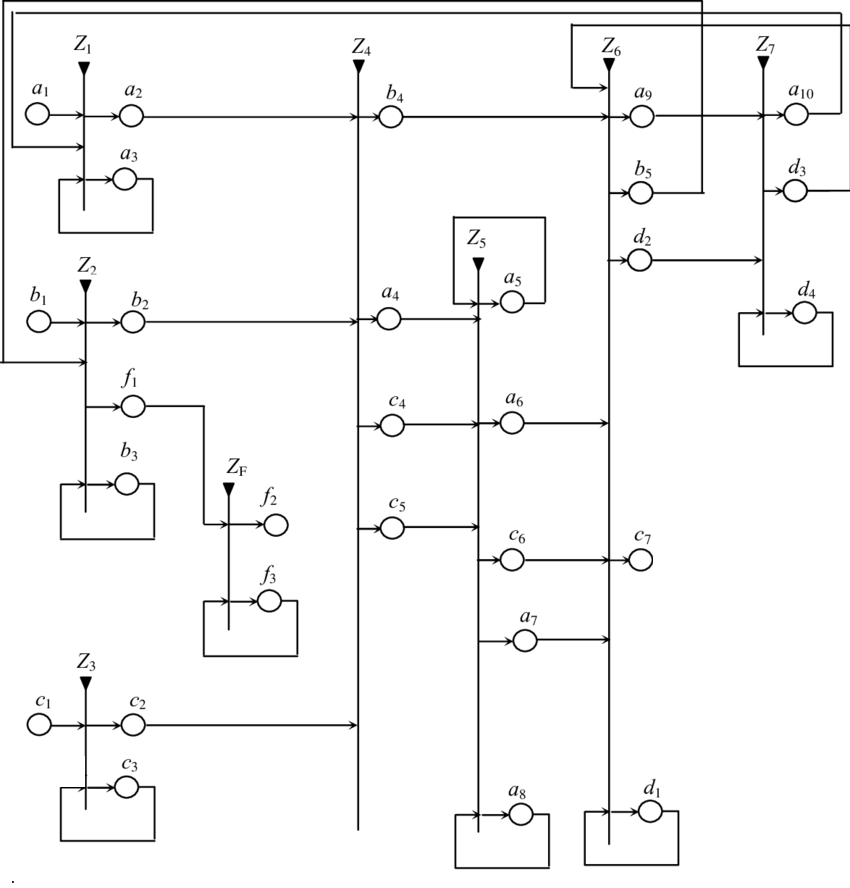
\includegraphics[width=0.65\linewidth]{2. algos/drawing/images/gen_net_example.png} \caption{Пример за чертеж на обобщена мрежа.} \label{fig:gen-net-example} \end{figure}

\subsubsection{Текущи практики при визуализирането на обобщени мрежи}

\hspace*{2.5em}Визуализирането на ОМ изисква прецизно позициониране на основните компоненти (позиции, преходи и ребра), което да гарантира яснота и структурна точност на модела. Традиционно този процес се осъществява чрез ръчно задаване на геометричните координати на всеки елемент. По-долу са разгледани утвърдените практики и конвенции, прилагани при ръчното графично оформяне на ОМ.

\paragraph{Насоченост на стрелките.} 
\mbox{}\\
В повечето ОМ стрелките, указващи движението между преходите и позициите, обичайно са ориентирани отляво надясно, тъй като това съвпада с естествената посока на четене. Тази ориентация подпомага ясното и интуитивно разбиране на потока и логиката на мрежата. Обичайно се следва стандарт, според който изходите на всеки преход се изобразяват вдясно. При необходимост се изобразяват и обратни преходи, но по начин, който не нарушава прегледността на графичната структура.

\paragraph{Позициониране на изходни позиции.}
\mbox{}\\
Основен акцент във визуализацията на ОМ е точното разположение на изходните позиции. Съгласно приетите конвенции за визуализация, всички изходни позиции се позиционират непосредствено вдясно на съответните преходи. По този начин се осигурява лесно проследяване на потока в мрежата, като графичните връзки сочат директно към съответните изходни позиции.

\paragraph{Позиции с двойна роля (вход и изход).}
\mbox{}\\
Обикновено дадена позиция в ОМ може да служи и като вход, и като изход за даден преход или за група от преходи. Когато позицията има такава двойна роля, тя се позиционира в долната част на прехода. Тази практика подпомага поддържането на подреден вид на диаграмата, като минимизира пресичането на ребра и предотвратява излишно визуално претоварване. Поставянето им в долната част на прехода допринася за по-ясно разграничение на отделните компоненти.

\paragraph{Допълнителни практики.}
\mbox{}\\
Освен изброените по-горе възприети конвенции, съществуват и други утвърдени подходи, които допринасят за по-добра четимост и последователност:

\begin{itemize} \item \textbf{Равномерни отстояния:} Поддържането на постоянни разстояния между елементите гарантира визуален баланс и улеснява интерпретацията. \item \textbf{Надписи:} Ясното и сбито етикетиране на позиции и преходи е от съществено значение. Надписите се поставят близо до съответните елементи, без да припокриват други части на мрежата. \item \textbf{Цветно разграничаване:} При необходимост се използва цветово маркиране за обозначаване на различните типове преходи или позиции, което внася допълнителна яснота. \item \textbf{Минимизиране на пресичанията:} Стремежът е да се сведат до минимум местата, където ребрата се пресичат, тъй като преплитащите се линии могат да затруднят недвусмисленото интерпретиране на диаграмата. Това се постига чрез внимателно планиране на разположението на елементите и на посоката на потока. \item \textbf{Последователна ориентация:} Общата ориентация на мрежата се поддържа непроменена в цялата диаграма. Това означава поддържане на движение отляво надясно и избягване на необосновани промени в посоката на ребрата, освен ако не са наложени от структурни особености на модела. \end{itemize}

Въпреки че тези практики допринасят за създаването на ясни и разбираеми диаграми, самият процес по ръчно задаване на координати за всеки елемент е трудоемък и податлив на грешки. Това подчертава необходимостта от автоматизирани решения, които да ускорят визуализацията и да гарантират точност и ефективност.

В следващите части се представя алгоритъм, предназначен да автоматизира процеса на чертане на ОМ. Той следва наложилите се практики за визуализация, като същевременно значително намалява ръчния труд и риска от допускане на грешки.

\subsubsection{Изчертаване на графи}

\hspace*{2.5em}Визуализацията на графи е основен подход при визуализацията и разбирането на сложни мрежи и взаимовръзки между обекти. То обединява методи от математиката, информатиката и визуализационните техники, за да представя графи в двумерно или тримерно пространство \cite{Kamada1989}. Ефективното графово чертане е от ключово значение за анализа на структури като социални и биологични мрежи, както и диаграми на потоци от данни.

Основната цел на графовото чертане е върховете и ребрата да се позиционират така, че структурата на графа да се възприема лесно, с минимален брой пресичания и с ясна визуализация на взаимовръзките. Съществуват редица алгоритми за постигане на оптимално подреждане, например методи за силово ориентиране (\textit{force-directed layouts}), йерархични (\textit{hierarchical layouts}) и кръгови (\textit{circular layouts}). Изборът на подходящ алгоритъм зависи от спецификите на графа и конкретното приложение, за което е предназначена визуализацията.

\paragraph{Изчертаване на графи с \textit{Graphviz}.} 
\mbox{}\\
\textit{Graphviz} е мощен инструмент с отворен код, разработен специално за визуализация на графи \cite{Ellson2004}. Той предоставя набор от методи за подреждане, подходящи за различни типове графи, което го прави изключително гъвкав. Чрез \textit{Graphviz} графите лесно се дефинират в текстов формат с езика \textit{DOT}, който впоследствие се обработва за генериране на визуални представяния.

\vspace{0.2cm}

Основните алгоритми за подреждане, предлагани от \textit{Graphviz}, включват:

\vspace{-0.4cm}

\begin{itemize} 
	\item \textbf{\textit{dot}}: Йерархичен алгоритъм за ориентирани графи, който организира върховете в слоеве. 
	\item \textbf{\textit{neato}}: Алгоритъм на силово ориентиране („пружинен“ модел), който позиционира върховете, подходящ предимно за неориентирани графи. 
	\item \textbf{\textit{fdp}}: Подобен на \textbf{\textit{neato}}, но използва различен метод за минимизиране на пресичанията между ребрата. 
	\item \textbf{\textit{twopi}}: Радиален алгоритъм, който разполага върховете в концентрични окръжности и често се използва за визуализиране на радиални йерархии. 
	\item \textbf{\textit{circo}}: Кръгов алгоритъм, особено полезен за циклични структури. 
\end{itemize}

С помощта на \textit{Graphviz} се генерират висококачествени визуални представяния на графи за широк спектър от приложения. Инструментът поддържа различни изходни формати (\textit{PNG, PDF, SVG} и др.), което улеснява интегрирането на резултатите в научни публикации и презентации. Освен това гъвкавостта на \textit{Graphviz} позволява персонализиране на формата на върховете, цветовете, стила на ребрата и други визуални елементи, като така се постигат естетични и информативни резултати при визуализацията.

Пример за резултат от автоматично генерирано изображение на граф с помощта на \textit{Graphviz} и алгоритъма \textit{dot} е показан на \textbf{Фигура~\ref{fig:Graphviz_first_example}}.
Йерархичното разположение на върховете ясно подчертава ориентираната структура на графа и минимизира визуалните пресичания между ребрата.\newpage


\begin{figure}[h!] \centering 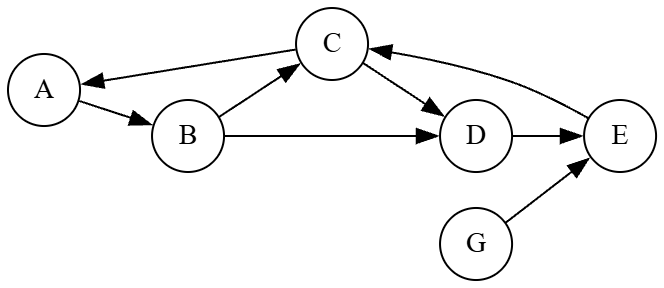
\includegraphics[width=0.9\textwidth]{2. algos/drawing/images//graphViz.png} \caption{Пример за граф, генериран чрез dot алгоритъма на \textit{Graphviz}.} \label{fig:Graphviz_first_example} \end{figure}

\subsubsection{Моделиране на обобщена мрежа като ориентиран граф}

\hspace*{2.5em}За да се визуализира и анализира структурата на ОМ, тя може да бъде представена като ориентиран граф. Такова графово представяне осигурява по-голяма яснота при проследяването на взаимовръзките между отделните компоненти на мрежата.

В контекста на теорията на графите:
\begin{itemize}[nosep]
    \item \textbf{Позициите} в ОМ се изобразяват като \textbf{върхове}. Всяка позиция отразява определено състояние или условие в системата.
    \item \textbf{Преходите} в ОМ също се изобразяват като \textbf{върхове}. Те отразяват процесите или действията, които предизвикват преминаване от едно състояние в друго.
    \item \textbf{Ребрата} (ориентирани ребра) представляват ориентирани връзки между върховете и отразяват потока в мрежата. Ребро се чертае от връх (позиция) към връх (преход), когато позицията е вход към този преход. По същия начин ребро се чертае от преход към позиция, когато позицията е негов изход.
\end{itemize}

В тази ориентирана графова структура ясно се проследява движението на \textbf{ядрата} (представящи обекти или информация) през ОМ, като посоката на ребрата отразява логиката на мрежата.

\paragraph{Пример.}
\mbox{}\\
Разглежда се ОМ с пет позиции и три прехода:
\begin{itemize}[nosep]
    \item \textbf{Позиции}: \(l_1\), \(l_2\), \(l_3\), \(l_4\), \(l_5\)
    \item \textbf{Преходи}: \(Z_1\), \(Z_2\), \(Z_3\)
\end{itemize}

Връзките в мрежата са:

\begin{itemize}[nosep]
    \item \(l_1 \rightarrow Z_1\)
    \item \(Z_1 \rightarrow l_2, l_3\)
    \item \(l_2 \rightarrow Z_2\)
    \item \(Z_2 \rightarrow l_4\)
    \item \(l_3, l_4 \rightarrow Z_3\)
    \item \(Z_3 \rightarrow l_5\)
\end{itemize}

В графовата интерпретация както позициите \((l_1, l_2, l_3, l_4, l_5)\), така и преходите \((Z_1, Z_2, Z_3)\) се разглеждат като \textbf{върхове} в графа. Насочените връзки се представят чрез ребра:

\begin{itemize}[nosep]
    \item Чертае се ориентирано ребро от \(l_1\) към \(Z_1\), тъй като \(l_1\) е вход към този преход.
    \item Чертаят се ребра от \(Z_1\) към \(l_2\) и \(l_3\), които обозначават изходите на прехода.
    \item От \(l_2\) се чертае ориентирано ребро към \(Z_2\), от който се чертае ребро към \(l_4\).
    \item Накрая от \(l_3\) и \(l_4\) се чертаят ребра към \(Z_3\), а от него се чертае ребро към \(l_5\).
\end{itemize}

Описаната по-горе ОМ е визуализирана на \textbf{Фигура~\ref{fig:gen-net-z1-z3}}. Тя представя позициите и преходите в съответствие с дефинираните връзки, като ясно се откроява последователността на потока и ролята на всеки преход в мрежата.

\vspace{0.4cm}

%this should be replaced with latex draw !!!
\begin{figure}[h!]
    \centering
    \tiny
    \begin{center}
    \setlength{\unitlength}{14pt}
    \begin{picture}(18.47,7.73)
    \linethickness{0.4pt}
    % --- Transitions ---
    \put(3.05,7.98){\makebox(0,0)[b]{$Z_1$}}
    \put(3.05,6.67){\makebox(0,0)[bb]{\Large$\bigtriangledown$}}
    \put(3.05,6.67){\line(0,-1){6.67}}
    \put(9.27,7.98){\makebox(0,0)[b]{$Z_2$}}
    \put(9.29,6.67){\makebox(0,0)[bb]{\Large$\bigtriangledown$}}
    \put(9.29,6.67){\line(0,-1){3.33}}
    \put(15.40,7.98){\makebox(0,0)[b]{$Z_3$}}
    \put(15.42,6.67){\makebox(0,0)[bb]{\Large$\bigtriangledown$}}
    \put(15.42,6.67){\line(0,-1){6.67}}
    % --- Places ---
    \put(6.19,5.36){\makebox(0,0)[cc]{$l_2$}}
    \put(6.19,4.47){\circle{1.0}}
    \put(6.19,2.69){\makebox(0,0)[cc]{$l_3$}}
    \put(6.19,1.80){\circle{1.0}}
    \put(12.40,5.36){\makebox(0,0)[cc]{$l_4$}}
    \put(12.40,4.47){\circle{1.0}}
    \put(18.47,2.69){\makebox(0,0)[cc]{$l_5$}}
    \put(18.47,1.80){\circle{1.0}}
    \put(0.00,5.36){\makebox(0,0)[cc]{$l_1$}}
    \put(0.00,4.47){\circle{1.0}}
    % --- Edges ---
    % Z1 -> l2
    \put(3.07,4.47){\vector(1,0){2.62}}
    % Z1 -> l3
    \put(3.07,1.80){\vector(1,0){2.62}}
    % Z2 -> l4
    \put(9.31,4.47){\vector(1,0){2.59}}
    % Z3 -> l5
    \put(15.45,1.80){\vector(1,0){2.52}}
    % l1 -> Z1
    \put(0.50,4.47){\vector(1,0){2.52}}
    % l2 -> Z2
    \put(6.69,4.47){\vector(1,0){2.58}}
    % l3 -> Z3
    \put(6.69,1.80){\vector(1,0){8.71}}
    % l4 -> Z3
    \put(12.90,4.47){\vector(1,0){2.50}}
    \end{picture}
    \end{center}
    \normalsize
    \caption{Обобщена мрежа с позиции \(l_1, l_2, l_3, l_4, l_5\) и преходи \(Z_1, Z_2, Z_3\).}
    \label{fig:gen-net-z1-z3}
\end{figure}

% \begin{figure}[h!]
%     \centering
%     
\includegraphics[width=0.8\textwidth]{algos/drawing/images//generatedGraph.png}
%     \caption{Ориентиран граф, отговарящ на дадената обобщена мрежа. Възлите представят позиции и преходи, а ориентираните дъги --- потока между тях.}
%     \label{fig:oriented_graph_example}
% \end{figure}

\vspace{0.6cm}

\begin{figure}[h!]
	\centering
	\begin{varwidth}{\textwidth}
		\centering
		\begin{tikzpicture}[
			node distance=0.4cm and 0.8cm,
			every node/.style={draw, shape=ellipse, minimum height=0.4cm, minimum width=0.8cm},
			->, >=Stealth
			]
			
			% Nodes
			\node (l1) {$l_1$};
			\node[right=of l1] (Z1) {$Z_1$};
			\node[above right=of Z1] (l2) {$l_2$};
			\node[right=of l2] (Z2) {$Z_2$};
			\node[right=of Z2] (l4) {$l_4$};
			\node[below right=of Z1] (l3) {$l_3$};
			\node[below right=of l4] (Z3) {$Z_3$};
			\node[right=of Z3] (l5) {$l_5$};
			
			% Arrows
			\draw (l1) -- (Z1);
			\draw (Z1) -- (l2);
			\draw (l2) -- (Z2);
			\draw (Z2) -- (l4);
			\draw (Z1) -- (l3);
			\draw (l4) -- (Z3);
			\draw (l3) -- (Z3);
			\draw (Z3) -- (l5);
		\end{tikzpicture}
		
		\captionsetup{width=0.6\linewidth, justification=centering}
		\caption{Ориентиран граф, съответстващ на обобщената мрежа. Върховете представляват позиции и преходи, а ориентираните ребра – потока между тях.}
		\label{fig:gen-network-graph}
	\end{varwidth}
\end{figure}

Както се вижда от примера, показан на \textbf{Фигура~\ref{fig:gen-network-graph}}, такова представяне на ОМ като ориентиран граф подпомага по-добрата визуализация на взаимодействията между позициите и преходите. Така се улеснява разбирането и анализа на поведението на системата.

\subsubsection{Визуализация на обобщени мрежи с \textit{Graphviz}}

\hspace*{2.5em}За ефективна визуализация на ОМ с помощта на \textit{Graphviz} е важно да се зададат параметри и ограничения, които гарантират едновременно естетична подредба и точно представяне на структурата. По-долу са описани основните стъпки и съображения за постигането на тази цел:

\paragraph{Задаване на глобални параметри.}
\mbox{}\\
В началото на файла за \textit{Graphviz} се дефинират общи настройки, които определят цялостния вид и подредба на графа:

\begin{itemize}
    \item \textit{rankdir=LR}: Този параметър указва, че графът се визуализира отляво надясно, което съответства на обичайната практика при ОМ, при която преходите са подредени хоризонтално, а позициите -- вертикално: входните отляво, а изходните отдясно на прехода.
    \item \textit{splines=ortho}: С тази настройка всички ребра стават ортогонални, т.е. сегментите им са успоредни на координатните оси (X и Y). Това е от особено значение за ОМ, защото съхранява ясната решетъчна структура, при която връзките са праволинейни и взаимно перпендикулярни, което улеснява визуалното възприемане.
\end{itemize}

\paragraph{Дефиниране на върховете за преходи.}
\mbox{}\\
Върховете, представящи преходи в ОМ, обикновено символизират действия или процеси и обичайно се изобразяват като правоъгълници или плътни линии. Реализацията в \textit{Graphviz} се постига чрез:

\begin{itemize}
    \item \textit{shape=rect}: Определя формата на върха (прехода) като правоъгълник за визуално разграничаване от кръглите или елиптичните върхове, представящи позиции.
    \item \textit{height=\{count of output places\}, width=0.05}: Височината на всеки правоъгълник се задава динамично според броя изходни позиции на прехода, а ширината се поддържа фиксирана на 0.05 инча (\textit{inches}), за да съответства на стандартното графично означение на прехода като вертикален сегмент. По този начин визуално се представя функционалността на прехода като структурен елемент, свързващ множество входни и изходни позиции.
\end{itemize}

\paragraph{Групиране на изходните позиции с \textit{subgraph}.}
\mbox{}\\
В \textit{Graphviz} изходните позиции обикновено се изобразяват непосредствено до съответния преход. За да се гарантира, че тези позиции са групирани и запазват относителното си разположение:

\begin{itemize}
    \item Дефинират се в \textit{subgraph cluster}. Чрез групиране на върха (прехода) и свързаните с него изходни позиции в \textit{subgraph}, те се  третират като логическа група по време на автоматичното подреждане. Така се избягва вероятността върховете да бъдат разместени или разделени при чертането на графа, като се запазва визуалното единство на ОМ.
    \item \textit{rank=same}: За да се осигури, че всички изходни върхове за даден преход са подравнени на еднаква височина (еднакво \textit{Y}-координатно ниво), се използва командата \textit{rank=same} в \textit{subgraph} клъстера. Това гарантира, че изходните позиции са хоризонтално подредени, което прави графа по-прегледен и по-лесен за тълкуване.
\end{itemize}

\paragraph{Управление на входните ребра чрез „невидими“ върхове.}
\mbox{}\\
Едно от предизвикателствата при използване на \textit{Graphviz} е дефинирането на единна входна точка (порт) за всички входящи ребра към даден преход. За да се постигне това, се въвежда концепцията за помощна структура („невидим“ връх) на прехода:

\begin{itemize}
    \item За всяко входно ребро към преходен връх се създава нов връх \textit{invisible\_node}, който се позиционира вляво от него.
    \item Входящата позиция се свързва с \textit{invisible\_node}, вместо директно с преходния връх.
    \item \textit{invisible\_node} се свързва с прехода чрез видимо ребро, като така се гарантира, че реброто влиза в прехода от лявата му страна.
    \item \textit{invisible\_node} и преходният връх се позиционират в общ \textit{subgraph cluster}, за да се запази относителното им разположение и да се избегне преместването им при автоматичното подреждане.
\end{itemize}

Чрез този подход се постига по-изчистен и подреден вид, при който всички входящи връзки към прехода изглеждат сякаш идват от точка вляво. Това не само подобрява визуалната четимост на диаграмата, но и улеснява възприемането на логическия поток на преходите. С помощта на невидими върхове и внимателното им позициониране обобщената мрежа се визуализира с ясна и последователна структура, което прави анализа и разбирането на потока в системата по-интуитивни.

Ефектът от използването на невидими върхове при подравняването на входните ребра към преходите е илюстриран на \textbf{Фигура~\ref{fig:after_optimization}}.

\begin{figure}[h!]
    \centering
    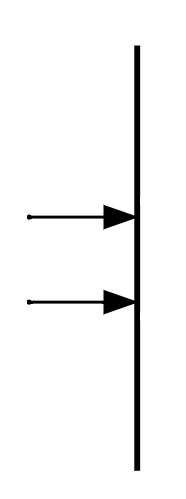
\includegraphics[width=0.15\textwidth]{2. algos/drawing/images//invis_nodes.png}
    \caption{Визуализация на преход с „невидим“ връх пред него.}
    \label{fig:after_optimization}
\end{figure}

\subsubsection{Алгоритъм за генериране на \textit{Graphviz} низове от обобщени мрежи}

\hspace*{2.5em}В този раздел се описва алгоритмичната логика за генериране на \textit{Graphviz} низ от ОМ (\textit{GN}). Алгоритъмът е създаден за автоматизиране на визуализацията на ОМ и гарантира, че полученият граф следва предварително зададените параметри на подредба. Основната функция, \textit{generateGraphvizString}, използва няколко спомагателни функции, които отговарят за картографирането на преходи и позиции, генерирането на невидими върхове и създаването на необходимите ребра между елементите в ОМ.

Структурата на псевдокода, обобщаваща основните стъпки и логиката на алгоритъма, е дефинирана по следния начин:

\paragraph{Генериране на невидими върхове.}
\mbox{}\\
Функцията \textit{genInvisNodes} генерира невидими върхове, използвани за подравняване на преходите при графичното подреждане на графа.

\begin{algorithm}[H]
\caption{genInvisNodes(result, genNet, transition)}
\begin{algorithmic}
\For{each inputPlace in transition}
    \State \texttt{result $\gets$ result + "invis\_node\_"{} + transition.name + "\_"{} + indexOf(inputPlace) + "[shape = point, width = 0.01, height = 0.01]"{} + newLine}
\EndFor
\end{algorithmic}
\end{algorithm}

\paragraph{Свързване на невидимите върхове с преходите.}
\mbox{}\\
Функцията \textit{genEdgeBetweenInvisNodesAndTransition} генерира ребра от невидимите върхове към преходите, като осигурява коректно подравняване и свързване.

\begin{algorithm}[H]
\caption{genEdgeBetweenInvisNodesAndTransition(result, genNet, transition)}
\begin{algorithmic}
\For{each inputPlace in transition}
    \State \texttt{result $\gets$ result + "invis\_node\_"{} + transition.name + "\_"{} + indexOf(inputPlace) + \detokenize{" -> "} +  transition.name + ":w"{} + newLine}
\EndFor
\end{algorithmic}
\end{algorithm}

\paragraph{Генериране на преходи.}
\mbox{}\\
Функцията \textit{genTransitionsString} генерира необходимата конфигурация за всеки преход в ОМ, включително невидимите върхове и връзките помежду им.

\begin{algorithm}[H]
\caption{genTransitionsString(genNet, result)}
\begin{algorithmic}
\For{each transition in genNet.transitions}
    \State \texttt{result $\gets$ result + "subgraph cluster\_"{} + transition.name + "\{"}
    \State \texttt{result $\gets$ result + "style=invis"}
    \State \texttt{result $\gets$ result + "subgraph cluster\_"{} + transition.name + "\_0"{} + "\{"}
    \State \texttt{result $\gets$ result + transition.name + 
    "[shape=rect, height=max(count(outputPlaces), count(inputPlaces)), width = 0.005]"}
    \State \texttt{call genInvisNodes(result, genNet, transition)}
    \State \texttt{call genEdgeBetweenInvisNodesAndTransition(result, genNet, transition)}
    \State \texttt{call genOutgoingPlacesFromTransition(result, genNet, transition)}
    \State \texttt{call genOutgoingEdgesFromTransition(result, genNet, transition)}

    \texttt{result $\gets$ result + "\}"}
\EndFor
\end{algorithmic}
\end{algorithm}

\paragraph{Генериране на изходни позиции и ребра.}
\mbox{}\\
Две отделни функции отговарят за генерирането на изходните позиции и съответните ребра. Така се гарантира, че ребрата между преходите и позициите се създават коректно.

\begin{algorithm}[H]
\caption{genOutgoingPlacesFromTransition(genNet, result, transition)}
\begin{algorithmic}
\State \texttt{result $\gets$ result + "\{rank = same;"}
\For{each outputPlace in transition}
    \State \texttt{result $\gets$ result + outputPlace.name + ";"}
\EndFor
\State \texttt{result $\gets$ result + "\}"}
\end{algorithmic}
\end{algorithm}

\begin{algorithm}[H]
\caption{genOutgoingEdgesFromTransition(genNet, result, transition)}
\begin{algorithmic}
\For{each outputPlace in transition}
    \State \texttt{result $\gets$ result + transition.name \detokenize{" -> "} outputPlace.name  }
\EndFor
\end{algorithmic}
\end{algorithm}

\paragraph{Генериране на изходни ребра от позициите.}
\mbox{}\\
Накрая функцията \textit{genOutputEdgesFromPlaces} генерира ребра, свързващи позициите към невидимите върхове, като така се осигурява коректното подравняване на преходите.

\begin{algorithm}[H]
\caption{genOutputEdgesFromPlaces(genNet, result)}
\begin{algorithmic}
\For{each place in genNet}
    \State \texttt{invisNodeIndex $\gets$ first invisible node index for the transition}
    \State \texttt{result $\gets$ result + place.name + \detokenize{" -> "} + "invis\_node\_"{} + "transitionName"{} + "\_"{} + invisNodeIndex + "[arrowhead=none]"}
\EndFor
\end{algorithmic}
\end{algorithm}

\paragraph{Главна функция за генериране на \textit{Graphviz} низ.}
\mbox{}\\
Главната функция \textit{genGraphvizString} обединява всички предходни функции, като се генерира пълният \textit{Graphviz} низ, представляващ ОМ.

\begin{algorithm}[H]
\caption{genGraphvizString(genNet)}
\begin{algorithmic}
\State \texttt{result $\gets$ "\ {digraph G} "}
\State \texttt{result $\gets$ result + "rankdir=LR;"}
\State \texttt{result $\gets$ result + "splines=ortho;"}
\State \texttt{call genTransitionsString(result, genNet)}
\State \texttt{call genOutputEdgesFromPlaces(result, genNet)}
\State \texttt{result $\gets$ result + "\}"}
\end{algorithmic}
\end{algorithm}

Резултатът от прилагането на описания алгоритъм за генериране на \textit{Graphviz} низ е показан на \textbf{Фигура~\ref{fig:gen-network-Graphviz}}. Визуализацията отразява автоматично генерираната структура на ОМ преди последваща графична обработка.


\begin{figure}[h!]
    \centering
    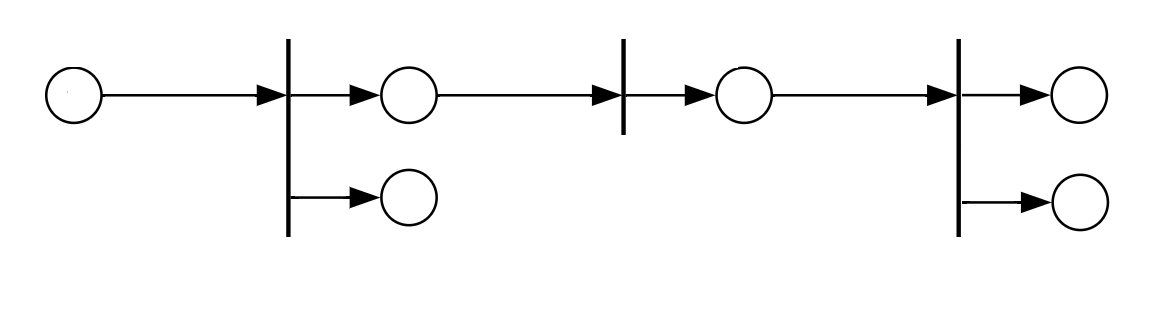
\includegraphics[width=\textwidth]{2. algos/drawing/images//genNetBeforePreprocess.png}
    \caption{Пример за визуализиран граф (обобщена мрежа) с помощта на Graphviz}
    \label{fig:gen-network-Graphviz}
\end{figure}

\paragraph*{Следваща обработка на генерираното изображение.}
\mbox{}\\
В този параграф се описват техниките, които се прилагат към \textit{SVG} (\textit{Scalable Vector Graphics}) файла, генериран от алгоритъма. Първоначално се създава граф, където преходите са представени като много тънки правоъгълни върхове, а позициите -- като кръгови върхове. За да се адаптира това визуално представяне към формата на ОМ (\textit{GN}), при последваща обработка се извършват редица модификации.

Целта е полученото изображение да съответства по-добре на формата на ОМ. По-долу са описани конкретните промени:

\begin{itemize}
    \item \textbf{Преходи:}  
    Всеки преход, първоначално дефиниран като тесен правоъгълник, подлежи на допълнителна обработка: в горната му част се добавя черен триъгълник, който служи за графичен идентификатор и подобрява неговата видимост в общата структура. Над триъгълника се визуализира етикет с наименованието на прехода, което гарантира неговата еднозначна идентификация в модела.

    \item \textbf{Позиции:}  
    При позициите, представени с окръжности, се добавят имената им над всяка окръжност. Това е необходимо, тъй като инструментът за генериране на първоначалния \textit{SVG} (\textit{Graphviz}) не поддържа по подразбиране този начин на надписване. Затова ръчно се вмъкват нужните надписи, за да се осигури яснота в крайното визуално представяне.
   

    \item \textbf{Визуализиране на обобщената мрежа:}  
    След прилагането на горните промени полученият \textit{SVG} значително наподобява ОМ. Преходите са ясно маркирани и надписани, а позициите (места) имат четливо поставени наименования над своите окръжности. Този подход води до по-интуитивна и точна графична репрезентация на системата, която се моделира, улеснявайки нейното тълкуване и анализ.
    
    Крайният резултат след прилагане на описаните стъпки за последваща \textit{SVG} обработка е показан на \textbf{Фигура~\ref{fig:gen-network-processed}}. Полученото изображение следва визуалните конвенции на ОМ и позволява интуитивно възприемане на структурата и потока.
    
	\newpage
    \item \textbf{Пример за резултатно изображение:}  
    \begin{figure}[h!]
        \centering
        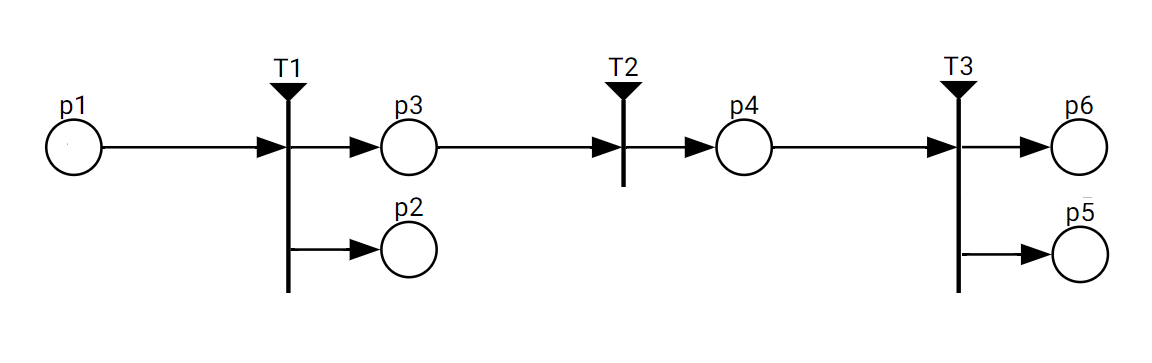
\includegraphics[width=\textwidth]{2. algos/drawing/images//genNetAfterPreprocess.png}
        \caption{Пример за визуализирана обобщена мрежа след обработка}
        \label{fig:gen-network-processed}
    \end{figure}

    \item \textbf{Псевдокод на стъпката по обработка:}

    \begin{algorithm}[H]
    \caption{postprocessSVG(graph)}
    \begin{algorithmic}
    \State \texttt{svg $\gets$ loadSVG(graph)}

    \For{each transition in svg}
        \State \texttt{points $\gets$ getTransitionPoints(transition)}
        \State \texttt{topPoint $\gets$ findTopMostPoint(points)}
        \State \texttt{addBlackTriangle(topPoint)}
        \State \texttt{label $\gets$ getTransitionLabel(transition)}
        \State \texttt{placeLabelAboveTriangle(topPoint, label)}
    \EndFor

    \For{each position in svg}
        \State \texttt{circle $\gets$ findCircle(position)}
        \State \texttt{centerPoint $\gets$ getCenterPoint(circle)}
        \State \texttt{label $\gets$ getPositionLabel(position)}
        \State \texttt{placeLabelAboveCircle(centerPoint, label)}
    \EndFor

    \State \texttt{outputSVG $\gets$ saveUpdatedSVG(svg)}
    \State \texttt{return outputSVG}
    \end{algorithmic}
    \end{algorithm}

    \item \textbf{Псевдокод на основната функция за чертане:}

    \begin{algorithm}[H]
    \caption{drawGenNet(genNet)}
    \begin{algorithmic}
    \State \texttt{graphvizStr $\gets$ genGraphvizString(genNet)}
    \State \texttt{svg $\gets$  Graphviz.render(graphvizStr)}
    \State \texttt{postprocessSVG(svg)}
    \end{algorithmic}
    \end{algorithm}
\end{itemize}